Stoffe können in verschiedenen Aggregatszuständen auftreten. Diese hängen von der Temperatur und dem Druck ab. Sie werden auch Phasen genannt. Abbildung \ref{Phasendiagramm} zeigt ein schematisches Phasendiagramm von Wasser. Liegt beispielsweise flüssiges Wasser vor, dann können Temperatur und Druck innerhalb des Phasenraums (also ohne überschreiten einer Linie) beliebig variiert werden, ohne den Aggregatszustand zu ändern.
\begin{figure}[ht!]
	\centering
	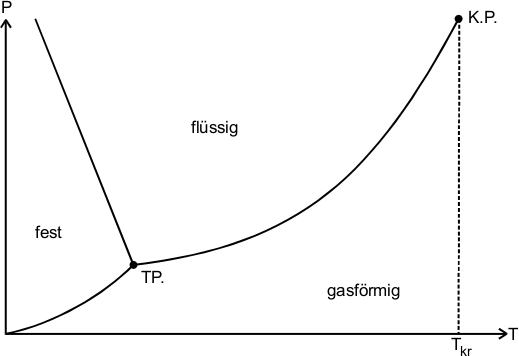
\includegraphics[width=0.9\textwidth]{Phasendiagramm.png}
	\caption{Phasendiagramm für Wasser\cite{V203}}
	\label{Phasendiagramm}
\end{figure} \\
Am Triple Punkt (TP) treten alle drei Phasen gleichzeitig auf. Die Kurve, die dort beginnt und die flüssige von der gasförmigen Phase trennt heißt Dampfdruckkurve. Hier hängen $p$ und $T$ voneinander ab. Diesen Zusammenhang beschreibt die Clausius-Clapeyronische Gleichung
\begin{equation}\label{Clausius}
	(V_\text{D}-V_\text{F})\ \text{d}p = \frac{L}{T}\ \text{d}T.
\end{equation}
Dabei ist $V_\text{D}$ das molare Volumen des Gases, $V_\text{F}$ das molare Volumen der Flüssigkeit, $T$ die Temperatur in Kelvin und $L$ die molare Verdampfungswärme. \\
Letztere ist die Menge Energie, die benötigt wird, um ein Mol Flüssigkeit bei konstanter Temperatur $T$ in Dampf umzuwandeln. $L$ ist abhängig vom Stoff und der Temperatur. In der Nähe des kritischen Punktes (siehe Abblidung \ref{Phasendiagramm}) verschwindet $L$, da es keinen Unterschied mehr zwischen flüssiger und gasförmiger Phase gibt. \\
Ist die Temperatur allerdings weit unter der kritischen Temperatur \[T_\text{Kr, Wasser} = \SI{374}{\celsius},\] kann $L$ als konstant betrachtet werden. Außerdem kann angenommen werden, dass $V_\text{F}$ vernachlässigbar gegenüber $V_\text{D}$ ist und $V_\text{D}$ der idealen Gasgleichung
\begin{equation}\label{ideales Gas}
	V_\text{D} = R\frac{T}{p}
\end{equation}
gehorcht. Dann vereinfacht sich die Clausius-Clapeyronische Gleichung zu
\begin{equation}\label{Clausius einfach}
	\frac{1}{p}\ \text{d}p = \frac{1}{R}\frac{L}{T^2}\ \text{d}T
\end{equation}
bzw. nach Integration
\begin{equation}\label{Regression ln(p)=1/T}
	\ln p = - \frac{1}{R}\frac{L}{T} + \frac{L}{RT_0}+\ln p_0.
\end{equation}